\section{Datenstrukturen}

Datenstrukturen dienen der strukturierten Speicherung von Daten, meist im Arbeitsspeicher.
Es soll schneller Zugriff und dass einfache Anwendungen von Algorithmen ermöglicht werden,
wobei es wichtig ist, dass die Datenstruktur zu den Daten passt.
Alle Beschreibungen der Datenstrukturen beziehen sich auf die Vorgaben des
Kerncurriculums Informatik.

\subsection{Statische Reihung}

Die statische Reihung (vgl. Array) speichert Daten eines Datentyps und hat
eine feste Länge. Der Zugriff auf die Daten erfolgt indexbasiert und
mit einer Zugriffszeit von $O(1)$.

\subsection{Dynamische Reihung}

Eine dynamische Reihung (vgl. std::vector/Python Liste) speichert Daten eines Datentyps und hat
eine variable Länge. Der Zugriff auf die Daten erfolgt indexbasiert und
mit einer Zugriffszeit von $O(1)$. Zusätzlich lassen sich Elemente an Position
entfernen oder einfügen, wodurch sich die anderen Elemente rechts davon verschieben.

\begin{table}[H]
    \begin{tabular}{|p{0.5\linewidth}|p{0.5\linewidth}|}
    \hline
    DynArray(): DynArray & Eine leere dynamische Reihung wird angelegt. \\ \hline
    isEmpty(): Wahrheitswert & Gibt True zurück, wenn die Reihung leer ist. \\ \hline
    getItem(Ganzzahl index): Inhalt & Gibt das Element am Index zurück. \\ \hline
    append(Inhalt inhalt) & Fügt ein Element am Ende hinzu. \\ \hline
    insertAt(Ganzzahl index, Inhalt inhalt) & Fügt ein Element am Index ein. Die Elemente rechts davon rücken um 1 Position nach rechts. \\ \hline
    setItem(Ganzzahl index, Inhalt inhalt) & Ersetzt das Element am Index. \\ \hline
    delete(Ganzzahl index) & Löscht das Element am Index, die anderen Elemente rücken nach links. \\ \hline
    getLength(): Ganzzahl & Gibt die Länge zurück \\ \hline
    \end{tabular}
\end{table}

\subsection{Schlange}

Eine Schlange (vgl. Queue) ist eine Datenstruktur mit variabler Länge, die nach dem
FIFO (First-in First-out) Prinzip funktioniert. Vergleichbar mit einer Warteschlange,
werden Elemente immer hinten hinzugefügt und von vorne entnommen. Die Zugriffszeit ist
$O(1)$ für das erste/letzte Element und sonst abhängig von der Position des gewollten
Elements in der Schlange.

\begin{table}[H]
    \begin{tabular}{|p{0.5\linewidth}|p{0.5\linewidth}|}
    \hline
    Queue() & Eine leere Schlange wird angelegt. \\ \hline
    isEmpty(): Wahrheitswert & Gibt True zurück, wenn die Schlange leer ist. \\ \hline
    head(): Inhalt & Gibt den Inhalt des ersten Element zurück, Element nicht entfernt. \\ \hline
    enqueue(Inhalt inhalt) & Hängt ein Element hinten an die Schlange an. \\ \hline
    dequeue(): Inhalt & Gibt den Inhalt des ersten Element zurück, Element entfernt. \\ \hline
    \end{tabular}
\end{table}

\subsection{Stapel}

Ein Stapel (vgl. Stack) ist eine Datenstruktur mit variabler Länge, die nach dem
LIFO (Last-in First-out) Prinzip funktioniert. Vergleichbar mit einem Stapel von Tellern,
lassen sich Elemente nur oben hinzufügen oder entfernen, aber nicht von unten.
Die Zugriffszeit ist $O(1)$ für das oberste Element und sonst abhängig davon, wie viele
Elemente über dem gewollten Element liegen.

\begin{table}[H]
    \begin{tabular}{|p{0.5\linewidth}|p{0.5\linewidth}|}
    \hline
    Stack() & Ein leerer Stapel wird angelegt. \\ \hline
    isEmpty(): Wahrheitswert & Gibt True zurück, wenn der Stapel leer ist. \\ \hline
    top(): Inhalt & Gibt den Wert des obersten Element zurück, Element wird nicht entfernt. \\ \hline
    push(Inhalt inhalt) & Legt ein Element oben auf den Stapel. \\ \hline
    pop(): Inhalt & Gibt den Wert des obersten Element zurück, Element wird entfernt.  \\ \hline
    \end{tabular}
\end{table}

\subsection{Binärbaum}

Ein Binärbaum ist eine nichtlineare Datenstruktur aus der Gruppe der Bäume, bei dem
jeder Knoten maximal 2 Unterknoten/Kinder hat. Das Hinzufügen, Entfernen und Auslesen
von Elementen des Baums ist dabei auf verschiedene Arten möglich.

\begin{figure}
    \centering
    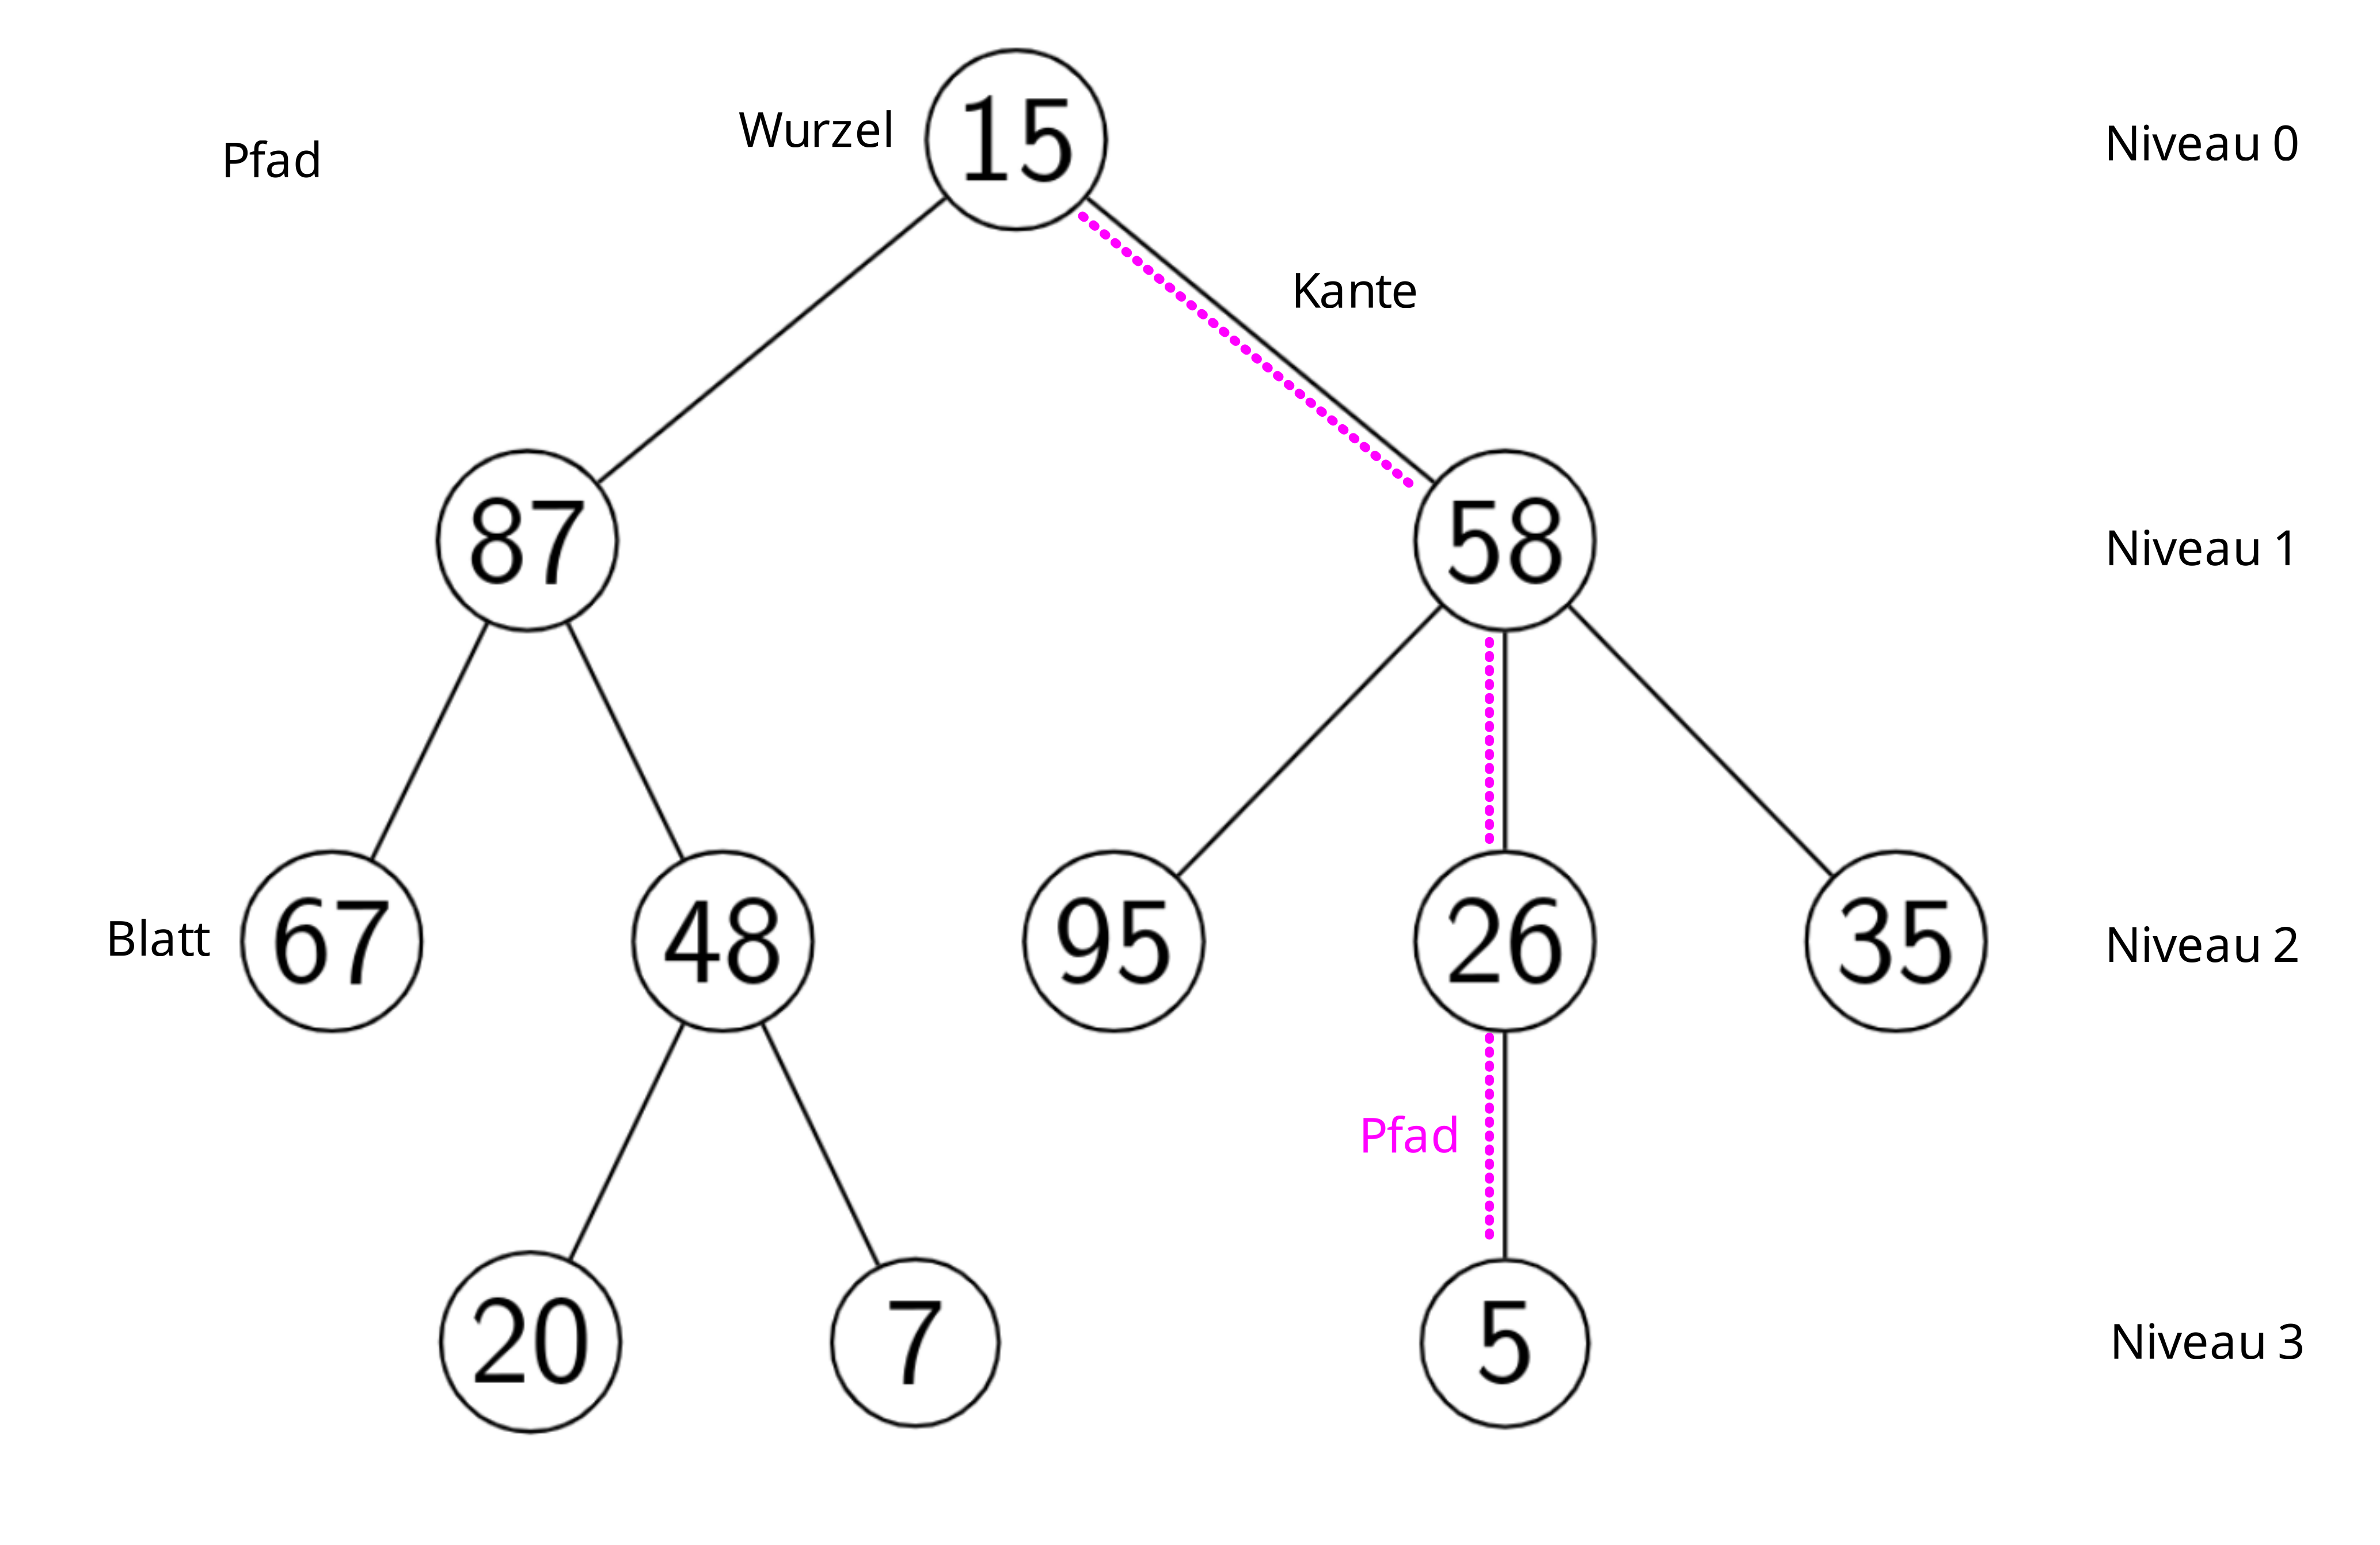
\includegraphics[width=1\textwidth]{images/baum_begriffe.png}
    \caption{Fachbegriffe bei Bäumen}
\end{figure}


\subsubsection{Traversierung von Binärbäumen}

Es gibt 3 gängige Verfahren zum Traversieren von Binärbaumen, um z. B. dann die Elemente
in einer anderen Datenstruktur (e.g. Schlange) zu speichern.
Alle 3 Varianten werden dabei Rekursiv beschrieben (eine Rekursive implementierung ist nicht nötig).

\vspace*{0.3cm}

\begin{forest}
    for tree={
        grow=south,
        circle, draw, minimum size=3ex, inner sep=1pt,
        s sep=7mm
    }
    [15
        [87
            [67]
            [48
                [20]
                [7]
            ]
        ]
        [58
            [95]
            [26
                [5]
            ]
            [35]
        ]
    ]
\end{forest}


\subsubsection*{Pre-Order}

1. Verarbeite den Wert der Wurzel

2. Führe Pre-Order auf den linken Teilbaum aus.

3. Führe Pre-Order auf den rechten Teilbaum aus.

\vspace*{0.5cm}

\begin{forest}
for tree={
    grow=south,
    circle, draw, minimum size=3ex, inner sep=1pt,
    s sep=7mm
}
[1
    [2
        [3]
        [4]
    ]
    [5
        [6]
        [7]
    ]
]
\end{forest}

\subsubsection*{In-Order}

1. Führe In-Order auf den linken Teilbaum aus.

2. Verarbeite den Wert der Wurzel

3. Führe In-Order auf den rechten Teilbaum aus.

\vspace*{0.5cm}

\begin{forest}
for tree={
    grow=south,
    circle, draw, minimum size=3ex, inner sep=1pt,
    s sep=7mm
}
[4
    [2
        [1]
        [3]
    ]
    [6
        [5]
        [7]
    ]
]
\end{forest}

\vspace*{0.3cm}

Ist der Binärbaum sortiert, sodass z. B. für jeden Teilbaum der Wert des linken 
Unterknotens kleiner und der des rechte Unterknotens größer ist als der Wert der Wurzel,
so werden die Elemente auf- bzw. absteigend sortiert durchlaufen.

\subsubsection*{Post-Order}

1. Führe Post-Order auf den linken Teilbaum aus.

2. Führe Post-Order auf den rechten Teilbaum aus.

3. Verarbeite den Wert der Wurzel

\vspace*{0.5cm}

\begin{forest}
for tree={
    grow=south,
    circle, draw, minimum size=3ex, inner sep=1pt,
    s sep=7mm
}
[7
    [3
        [1]
        [2]
    ]
    [6
        [4]
        [5]
    ]
]
\end{forest}
